\subsection{Pole-zero compensation di una sonda}

La \textit{pole-zero compensation} è una tecnica che permette di effettuare misure precise di circuiti ad alta impedenza e ad alte frequenze senza interferenze da parte dell'apparato di misura.
L'alta impedenza determina una forte dipendenza dalla frequenza in quanto, se determinata da grandi resistenze, subentrano induttanze parassite oppure è generata direttamente da piccole capacità.

\begin{wrapfigure}[6]{r}{0.45\textwidth}
\centering
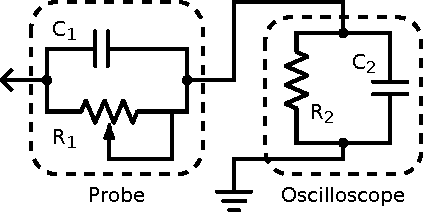
\includegraphics[width=.35\textwidth]{../E08/latex/probe.pdf}
\caption{Schema del circuito di misura composto dall'oscilloscopio e dalla sonda.}
\label{cir8:probe}
\end{wrapfigure}
